\documentclass[tikz,border=12pt]{standalone}
\usepackage{fontspec}
\setmainfont{Segoe UI}
\usepackage{amsmath,amssymb}
\usepackage{tikz}

\usetikzlibrary{calc,arrows.meta}

\begin{document}
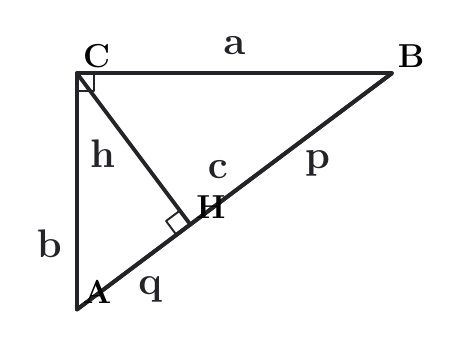
\begin{tikzpicture}[x=1.0000cm,y=1cm,line cap=round,line join=round]
\definecolor{linec0}{RGB}{35,35,40}
\definecolor{linec1}{RGB}{35,35,40}
\definecolor{linec2}{RGB}{35,35,40}
\definecolor{linec3}{RGB}{35,35,40}
\definecolor{linec4}{RGB}{35,35,40}
\definecolor{linec5}{RGB}{35,35,40}
\definecolor{edgecol}{RGB}{35,35,40}
\definecolor{hicol}{RGB}{35,35,40}
\definecolor{angcol}{RGB}{35,35,40}
\coordinate (C) at (0.0000,3.0000);
\coordinate (B) at (4.0000,3.0000);
\coordinate (A) at (0.0000,0.0000);
\coordinate (H) at (1.4400,1.0800);
\draw[line width=1.4pt,color={rgb,255:red,35;green,35;blue,40}] (A) -- (B);
\draw[line width=1.4pt,color={rgb,255:red,35;green,35;blue,40}] (B) -- (C);
\draw[line width=1.4pt,color={rgb,255:red,35;green,35;blue,40}] (C) -- (A);
\draw[line width=1.4pt,color={rgb,255:red,35;green,35;blue,40}] (C) -- (H);
\draw[line width=1.4pt,color={rgb,255:red,35;green,35;blue,40}] (H) -- (A);
\draw[line width=1.4pt,color={rgb,255:red,35;green,35;blue,40}] (H) -- (B);
\draw[edgecol,line width=0.7pt] (0.000,2.780) -- (0.220,2.780) -- (0.220,3.000);
\draw[edgecol,line width=0.7pt] (1.308,1.256) -- (1.132,1.124) -- (1.264,0.948);
\node[font=\bfseries\Large,text={rgb,255:red,35;green,35;blue,40}] at (2.000,3.350) {a};
\node[font=\bfseries\Large,text={rgb,255:red,35;green,35;blue,40}] at (-0.350,0.840) {b};
\node[font=\bfseries\Large,text={rgb,255:red,35;green,35;blue,40}] at (0.930,0.260) {q};
\node[font=\bfseries\Large,text={rgb,255:red,35;green,35;blue,40}] at (3.058,1.856) {p};
\node[font=\bfseries\Large,text={rgb,255:red,35;green,35;blue,40}] at (1.790,1.780) {c};
\node[font=\bfseries\Large,text={rgb,255:red,35;green,35;blue,40}] at (0.325,1.984) {h};
\node[font=\bfseries\large,inner sep=2pt,anchor=south west] at (0.000,3.000) {C};
\node[font=\bfseries\large,inner sep=2pt,anchor=south west] at (4.000,3.000) {B};
\node[font=\bfseries\large,inner sep=2pt,anchor=south west] at (0.000,0.000) {A};
\node[font=\bfseries\large,inner sep=2pt,anchor=south west] at (1.440,1.080) {H};
\end{tikzpicture}
\end{document}
